\documentclass[a4paper,10pt]{article}
\usepackage[polish]{babel}
\usepackage[utf8]{inputenc}
\usepackage{polski}
\usepackage[T1]{fontenc}
\usepackage{enumerate}
\usepackage{indentfirst}
\usepackage{graphicx}
\usepackage{fancyhdr}
\usepackage{minted}
\usepackage[pdftex,pagebackref=false,draft=false,pdfpagelabels=false,
colorlinks=true,urlcolor=blue,linkcolor=red,citecolor=green,pdfstartview=FitH,
pdfstartpage=1,pdfpagemode=UseOutlines,bookmarks=true,bookmarksopen=true]{hyperref}


\setlength{\textheight}{24cm}
\setlength{\textwidth}{15.92cm}
\setlength{\footskip}{10mm}
\setlength{\oddsidemargin}{0mm}
\setlength{\evensidemargin}{0mm}
\setlength{\topmargin}{0mm}
\setlength{\headsep}{5mm}

\definecolor{code}{rgb}{0.95,0.95,1}

\renewenvironment{description}[1][0pt]
	{\list{}{\labelwidth=0pt \leftmargin=#1
	\let\makelabel\descriptionlabel}}
	{\endlist}

\author{Mateusz Gałażyn, Jeremi Niedziela}
\title{Krótki kurs tworzenia stron w technologii PHP}


\frenchspacing
\begin{document}

\pagestyle{fancy}
\lhead{Krótki kurs tworzenia stron w technologii PHP}


\maketitle
\section{Wstęp}
Ten krótki kurs ma na celu przedstawienie sposobu pisania stron przy użyciu technologii Apache + MySQL + PHP (w skrócie AMP) - jednego z najpopularniejszych zestawów oprogramowania służącego do uruchamiania serwisów WWW. Ten kurs jest bardzo okrojony i zawiera tylko wybrane elementy języka PHP oraz MySQL dlatego aby w pełni zrozumieć metodykę tworzenia aplikacji w oparciu o te  języki dobrze jest się wspierać dokumentacjami technicznymi, innymi kursami dostępnymi w internecie, a także specjalistycznymi forami dyskusyjnymi. \\
Dokumentacja PHP: \href{http://www.php.net/manual/pl/}{http://www.php.net/manual/pl/} \\
Dokumentacja MySQL: \href{http://dev.mysql.com/doc/refman/5.5/en/index.html}{http://dev.mysql.com/doc/refman/5.5/en/index.html} \\
Dokumentacja Apache: \href{http://httpd.apache.org/docs/2.4/}{http://httpd.apache.org/docs/2.4/} \\
Kurs PHP @ Wikibooks: \href{http://pl.wikibooks.org/wiki/PHP}{http://pl.wikibooks.org/wiki/PHP}

\subsection{Mechanizm działania systemu AMP} 
Gdy użytkownik strony uruchamia przeglądarkę i wpisuje w pasek adresu, adres szukanego serwisu WWW, przeglądarka nawiązuje połączenie z serwerem na którym są uruchomione usługi umożliwiające dostęp do strony. \\
\textbf{Apache} - jest to najszerzej stosowany w internecie serwer HTTP \\
\textbf{PHP} - jeden z najpopularniejszych języków programowania używany do tworzenia stron WWW. \\
\textbf{MySQL} - system zarządzania bazami danych za pomocą języka SQL \\


\begin{figure}[htbp]
\centering
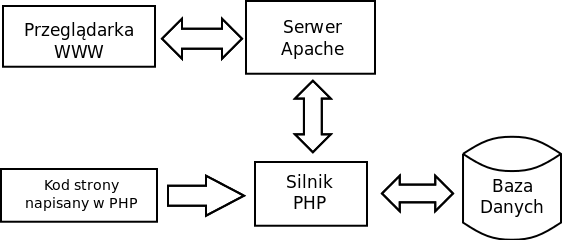
\includegraphics[width=0.7\textwidth]{LAMP.png}
\caption{Schemat komunikacji zestawu AMP}
\end{figure}

Żądanie otrzymane od przeglądarki jest przechwytywane przez serwer Apache, który przetwarzając je uruchamia kod strony napisany w języku PHP. Następnie silnik PHP  komunikuje się z bazą danych, pobiera dane, przetwarza je i zamienia na kod HTML, który zwraca serwerowi Apache. W kolejnym kroku serwer Apache wysyła kod HTML razem z obrazami umieszczonymi na stronie i stylami do przeglądarki, która renderuje i wyświetla stronę.

\section{Instalacja środowiska AMP}
\subsection{Instalacja na systemie Windows}
\subsubsection{Instalacja serwera Apache}
\subsubsection{Instalacja PHP}
\subsubsection{Instalacja serwera MySQL}
\subsection{Instalacja na systemie Linux}
\subsubsection{Instalacja serwera Apache}
\subsubsection{Instalacja PHP}
\subsubsection{Instalacja serwera MySQL}
\subsection{Konfiguracja}
\subsubsection{Konfiguracja Apache}
\subsubsection{Konfiguracja PHP}
%TODO konfiguracja timezone
%TODO ustawienie error_level i notice
\subsubsection{Konfiguracja MySQL}
% ustawianie hasła roota
\subsection{Instalacja phpMyAdmin}
% opis instalacji jak i interfejsu
\section{Projekt forum dyskusyjnego}
Naszym celem jest jest zbudowanie prostego forum dyskusyjnego. Musimy dać możliwość rejestrowania się poszczególnym użytkownikom, dodawania własnych wątków oraz odpowiadania na już utworzone. Potrzebne będzie też konto administratora, który będzie miał prawo moderacji odpowiedzi w tematach (postów).
\subsection{Układ podstron}
Gdy zostanie już ustalona lista wymaganych funkcjonalności projektowanego serwisu, następnym etapem jest stworzenie układu poszczególnych podstron.
\paragraph{Strona główna} Tutaj trzeba wyświetlić listę tematów (wraz z odnośnikami do podstrony, na którym będzie pojedynczy wątek wyświetlany w całości) które zostały założone na forum, umieścić odnośniki do podstrony z formularzem używanym do zalogowania się i rejestracji dla użytkowników oraz odnośnik do podstrony umożliwiającej założenie nowego tematu.
\paragraph{Podstrona wątku} W tym miejscu trzeba wyświetlić wszystkie posty w danym wątku, oraz formularz dający możliwość odpowiedzi w tym wątku. Gdy administrator wejdzie na tą podstronę, trzeba dać także dodatkowe możliwości edycji i usuwania poszczególnych postów.
\paragraph{Podstrona logowania} Zawierać będzie formularz logowania umożliwiający uwierzytelnienie użytkownika wchodzącego stronę. Uwierzytelnienie będzie polegało na porównaniu nazwy użytkownika i hasła z obecnymi w bazie danych. Po zalogowaniu się, użytkownik zostanie przekierowany z powrotem na stronę główną. Podstrona dostępna tylko dla niezalogowanych użytkowników.
\paragraph{Podstrona rejestracji} Odpowiedzialna za obsługę rejestracji nowego użytkownika. Trzeba będzie wyświetlić formularz rejestracji, odebrać i zweryfikować dane oraz dodać je do bazy danych.

\paragraph{Podstrona nowego wątku} Podstrona z formularzem umożliwiającym dodanie nowego wątku. Po odebraniu danych od użytkownika trzeba będzie dokonać ich weryfikacji i dodać do bazy danych. Na koniec trzeba przekierować użytkownika do podstrony wątku.

\paragraph{Podstrona edycji postu} Podstrona z formularzem umożliwiającym edycję własnych postów, a także w przypadku administratora - edycji każdego postu. Przekierowuje z powrotem do podstrony wyświetlającej cały wątek. \\

\begin{figure}[htbp]
\centering
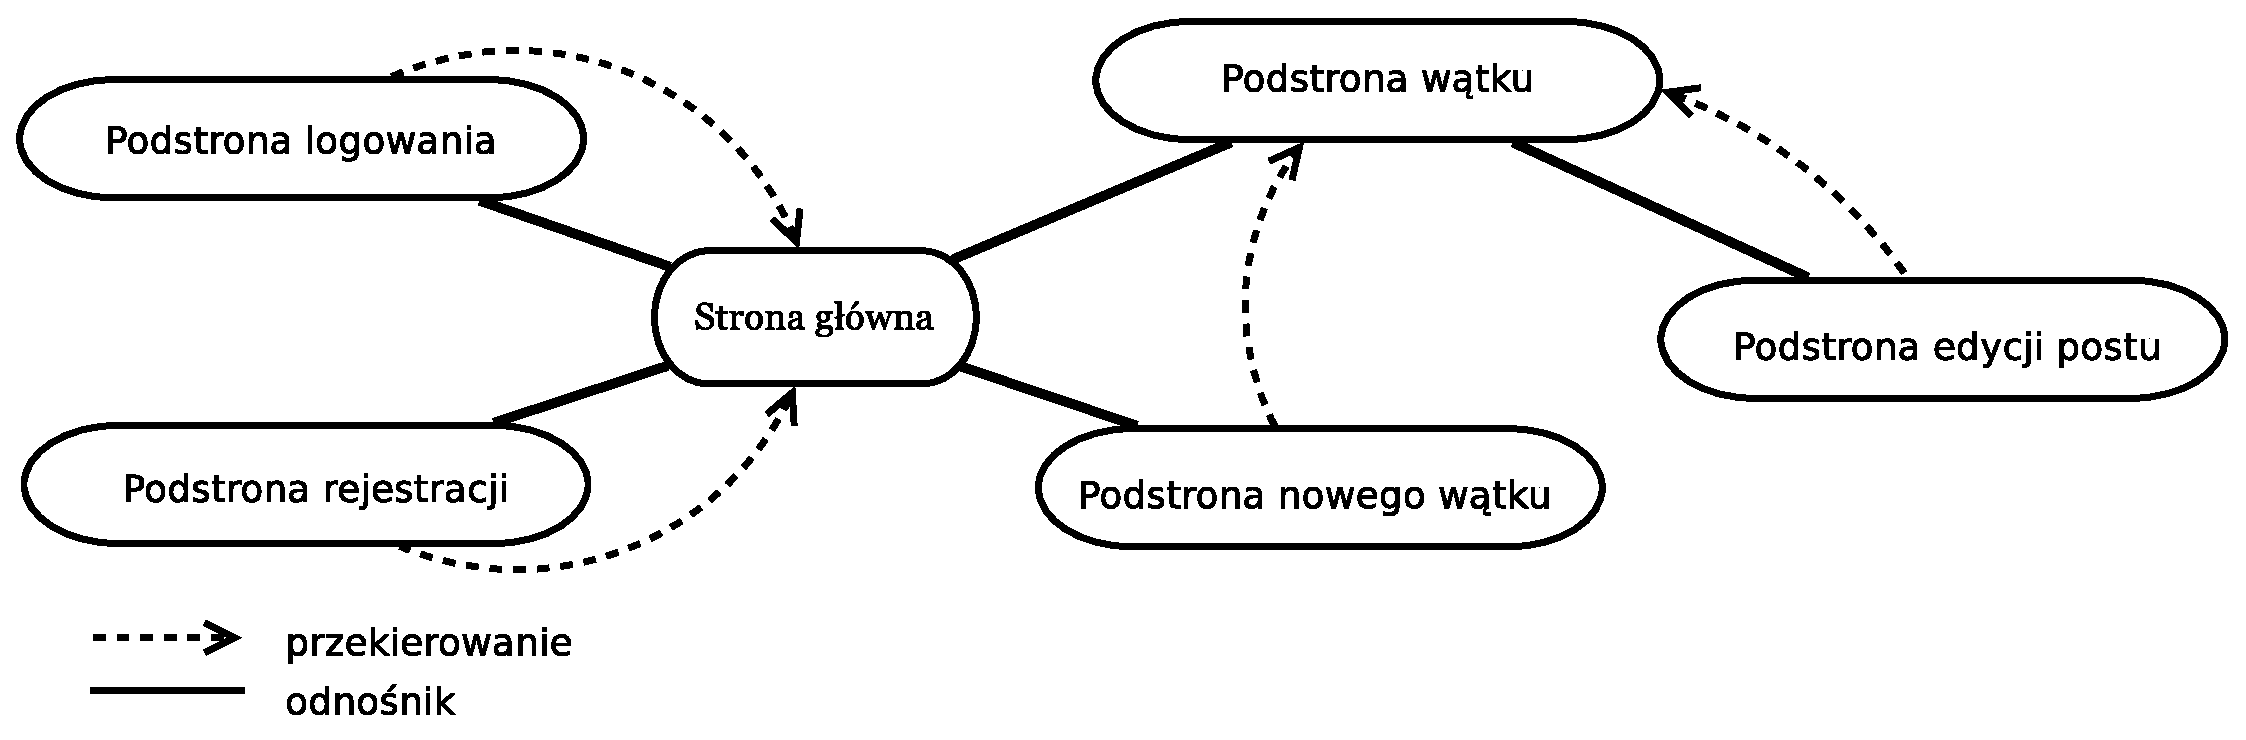
\includegraphics[width=0.9\textwidth]{subp.eps}
\caption{Układ podstron forum}
\end{figure}


\subsection{Projekt bazy danych}
Informacje w bazie danych są przechowywane w postaci tabel, podobnie jak w arkuszach kalkulacyjnych dostępnych w popularnych pakietach biurowych. W bazie projektowanego forum będziemy przechowywać listę użytkowników, listę tematów oraz listę postów. Dla każdej z tych list trzeba utworzyć oddzielną tabelę: users, threads, posts. W każdej z tych tabel konieczne jest stworzenie odpowiednich kolumn służących do przechowywania danych we właściwych typach. Ustawienie typu danej przechowywanej w każdej kolumnie przyśpiesza pracę serwera MySQL poprzez automatyczną optymalizację realizowanych zapytań do bazy oraz optymalizację sposobu przechowywania tabel na dysku.
\subsubsection{Typy danych MySQL}
W języku MySQL jest wiele typów danych 
(dokładny opis: \href{http://dev.mysql.com/doc/refman/5.5/en/data-type-overview.html}{http://dev.mysql.com/doc/refman/5.5/en/data-type-overview.html}), te najważniejsze to:

\paragraph{Typy znakowe:}
\begin{description}[5mm]
\item[CHAR] Przechowuje ciąg znaków do 255 elementów.
\item[VARCHAR] Tak jak \textbf{CHAR} przechowuje ciąg znaków do 255 elementów. Główną różnicą pomiędzy nimi jest to, że \textbf{VARCHAR} zmienia swój rozmiar w zależności od przyjętej liczby znaków, a \textbf{CHAR} zawsze rezerwuje miejsce 255 znaków niezależnie od długości zapisywanego ciągu.
\item[TEXT] Przechowuje ciąg do 65535 znaków.
\item[MEDIUMTEXT] Przechowuje ciąg do 16777215 znaków.
\end{description}

\paragraph{Typy liczbowe:}
\begin{description}[5mm]
\item[TINYINY] Przechowuje liczby od -128 do 127 (0 do 255 w przypadku \textbf{UNSIGNED}).
\item[SMALLINT] Przechowuje liczby od -32768 to 32767 (0 do 65535 w przypadku \textbf{UNSIGNED}).
\item[MEDIUMINT] Przechowuje liczby od -8388608 do 8388607 (0 do 16777215 w przypadku \textbf{UNSIGNED}).
\item[FLOAT] Małe liczby zmiennoprzecinkowe.
\item[DOUBLE] Liczby zmiennoprzecinkowe o podwojonej precyzji.
\end{description}
Każdy typ liczbowy występuje także w wersji \textbf{UNSIGNED}, która pozwala przechowywać dwa razy większe liczby bez przechowywania informacji o znaku.
\paragraph{Inne typy:}
\begin{description}[5mm]
\item[DATE] Data w formacie YYYY-MM-DD
\item[DATETIME] Data w formacie YYYY-MM-DD HH:MM:SS
\item[TIMESTAMP] Znacznik czasu w formacie: YYYYMMDDHHMMSS
\item[TIME] Czas w formacie: HH:MM:SS
\item[ENUM] Podobnie jak w C++, definiuje listę określonych wartości jakie może przyjąć to pole.
\item[SET] Podobnie jak \textbf{ENUM}, lecz pole w tabeli może przyjąć kilka wartości na raz.
\end{description}

\subsubsection{Projekty tabel}
Tabela \textit{users} powinna zawierać kolumny przechowujące informacje o użytkowniku takie jak: nazwa użytkownika, login używany przy identyfikacji na stronie, hash SHA-1\footnote{W bazach danych \textbf{NIGDY} nie powinno się przechowywać haseł w jawnej postaci tekstu. W przypadku gdy osoba trzecia uzyska nieautoryzowany dostęp do bazy danych, będzie mogła skopiować listę haseł wszystkich użytkowników, co nie powinno mieć nigdy miejsca. Zamiast tego przechowuje się specjalne hashe wygenerowane na podstawie haseł. Więcej informacji na temat hashy: \href{http://pl.wikipedia.org/wiki/Funkcja_skrótu}{pl.wikipedia.org}} hasła oraz pole determinujące czy dany użytkownik ma uprawnienia administracyjne (wartość 1, gdy użytkownik jest administratorem). \\
Tabela \textit{threads} powinna zawierać kolumny przechowujące tytuł wątku, zawartość pierwszego posta oraz data utworzenia wątku. \\
Tabela \textit{posts} powinna zawierać kolumny przechowujące treść posta i datę jego utworzenia. \\
Dodatkowo w każdej z tabel powinna znajdować się kolumna \textit{id} identyfikująca w każdej tabeli pojedynczy rekord. To rozwiązania ułatwia odwoływanie się do poszczególnych wpisów (rekordów)  w tabeli, bez konieczności ponownego przeszukiwania całej tabeli.
W tabelach \textit{posts} i  \textit{threads} oprócz informacji o postach i wątkach musimy utworzyć tak zwane relacje - kolumny wiążące poszczególne posty z użytkownikami oraz wątkami. Jest to tak zwana relacja \textbf{jeden do wielu}. Zagadnienie to można rozwiązać w prosty sposób: w tabeli \textit{threads} tworzymy kolumnę \textit{author\_id}, którą będzie zawierała id rekordu w tabeli \textit{users} odpowiadającego użytkownikowi, który stworzył dany wątek. Analogiczną operację trzeba wykonać dla tabeli posts: tworzymy kolumnę \textit{author\_id} oraz dodatkową \textit{thread\_id}, która definiuje wątek do którego przynależy dany post.

\begin{figure}[htbp]
\centering
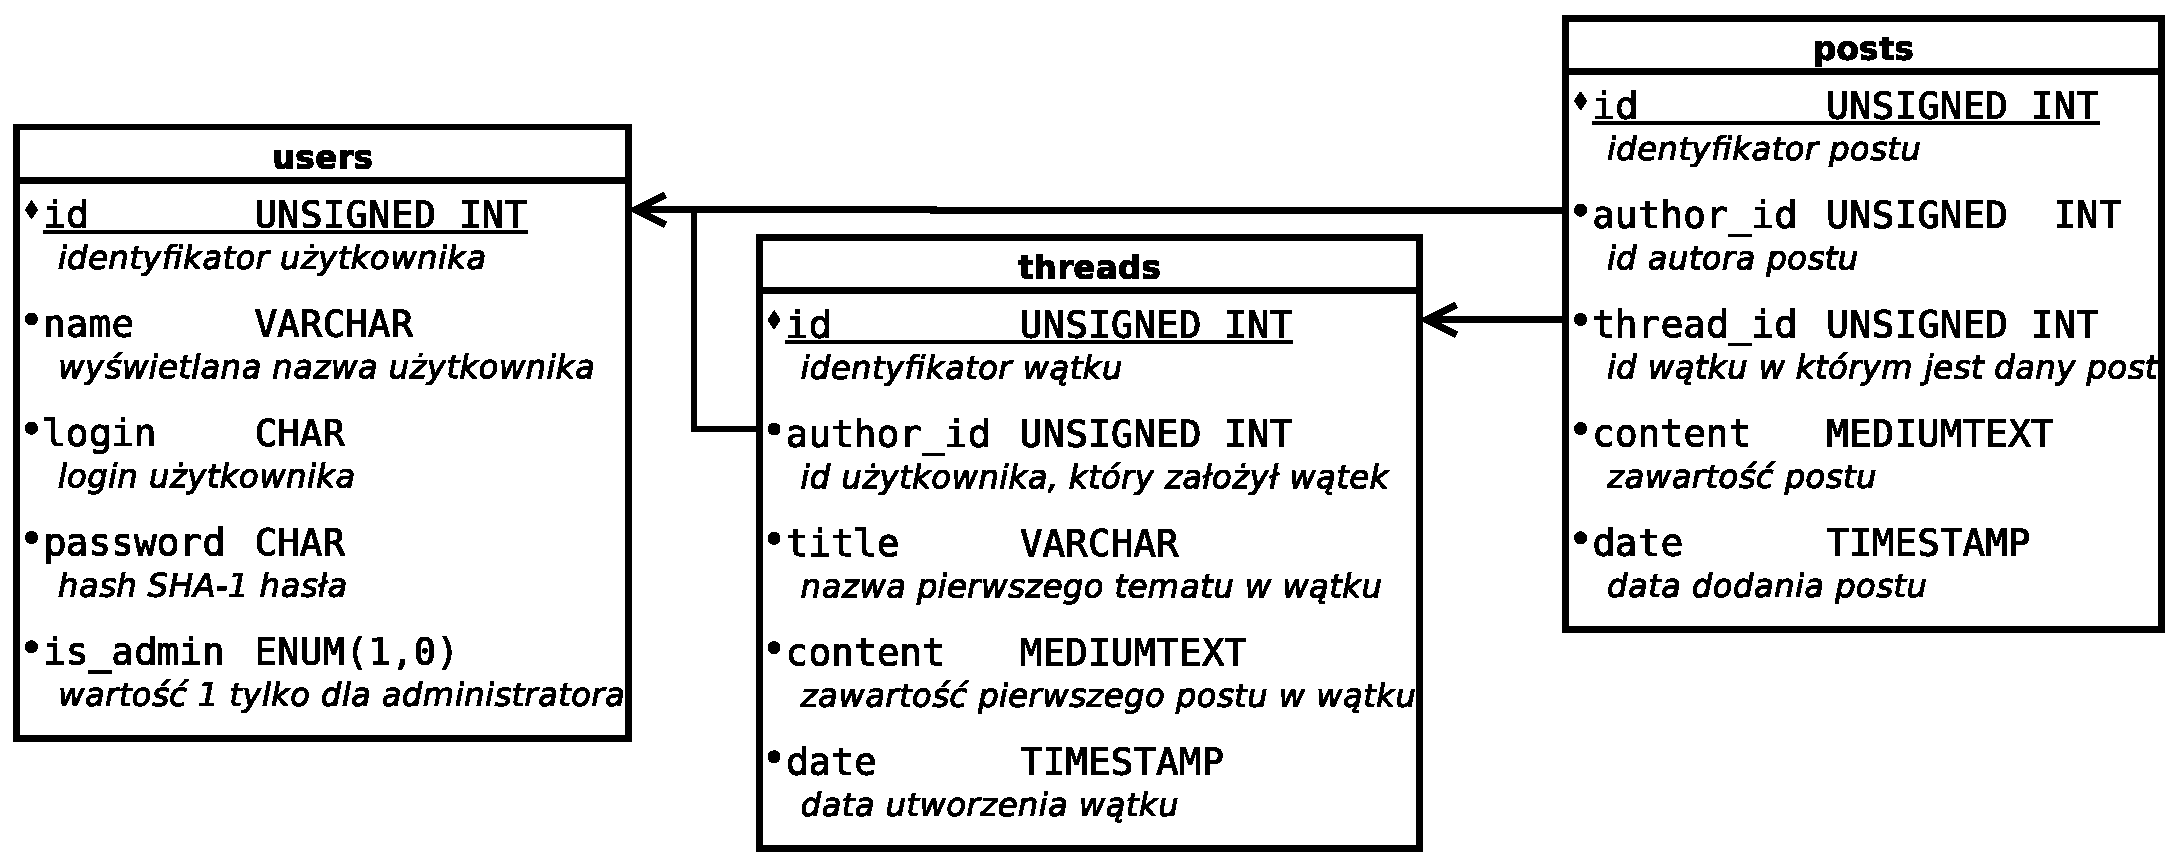
\includegraphics[width=1\textwidth]{db.eps}
\caption{Schematy tabel i ich wzajemne relacje}
\end{figure}

\paragraph{Optymalizacja}
Oprócz precyzowania typów danych dla każdej kolumny, aby ułatwić sobie i serwerowi pracę można zdefiniować dodatkowe atrybuty dla poszczególnych kolumn. Kolumna \textit{id} występująca w każdej z tabel musi być zdefiniowana z atrybutami \textit{PRIMARY KEY} (co jest zaznaczone na schemacie podkreśleniem) - oznacza to, że kolumna jest wykorzystywana do identyfikacji rekordów w tabeli, \textit{AUTO\_INCREMENT} - każdy dodawany rekord ma ustawiane automatycznie \textit{id} o 1 większe niż największe \textit{id} w tabeli, \textit{NOT NULL} - nie może mieć wartości 0.

\subsubsection{Kod SQL}
Nadszedł czas na stworzenie zaprojektowanej przez nas struktury tabel. Uruchamiamy serwer MySQL, a następnie poleceniem (dla systemu Linux): \\
\begin{minted}[bgcolor=code]{bash}
mysql -u root -p
\end{minted}
uruchamiamy wiersz poleceń MySQL.
Na systemie Windows aby uruchomić wiersz poleceń, wpierw trzeba uruchomić terminal, a w nim wpisać:  \\
\begin{minted}[bgcolor=code]{bat}
C:> cd C:\sciezka\do\katalogu\mysql\bin
C:\sciezka\do\katalogu\mysql\bin> mysql.exe -u root -p
\end{minted}
Następnie po wpisaniu hasła, aby stworzyć bazę danych wydajemy polecenie: \\
\begin{minted}[bgcolor=code]{sql}
CREATE DATABASE forum;
\end{minted}
Aby przystąpić do tworzenia tabel, trzeba wybrać nowo utworzoną bazę danych: \\
\begin{minted}[bgcolor=code]{sql}
USE forum;
\end{minted}
Możemy teraz utworzyć tabelę \textit{users} wydając poniższe polecenie: \\
\begin{minted}[linenos=true, bgcolor=code]{sql}
CREATE TABLE `forum`.`users` (
	`id` INT UNSIGNED NOT NULL AUTO_INCREMENT PRIMARY KEY ,
	`name` VARCHAR( 255 ) NOT NULL ,
	`login` CHAR( 255 ) NOT NULL ,
	`password` CHAR( 255 ) NOT NULL ,
	`is_admin` ENUM( '1', '0' ) NOT NULL ,
	UNIQUE (
		`name` ,
		`login` 
	)
);
\end{minted}
Ważne jest umieszczenie na końcu wyrażenia średnika, ponieważ informuje to interpreter MySQL że to jest koniec komendy. Bez średnika interpreter będzie czekał na dalsze wprowadzanie komend, dopóki nie napotka średnika.
W linii 1 podajemy nazwę bazy danych, a po kropce jest nazwa tworzonej tabeli. Nazwy bazy, tabel i kolumn są wzięte w ` `. W liniach 2-6 zdefiniowane są kolumny tabeli oddzielone przecinkami. Składnia jest następująca: \\
\begin{minted}[bgcolor=code]{sql}
`nazwa_kolumny` TYP NULL [dodatkowe atrybuty] ,
\end{minted}
Na początku podajemy nazwę kolumny, potem nazwę typu, jeżeli jest to typ liczbowy bez znaku, za nazwą typu dodajemy \textit{UNSIGNED}. Jeżeli jest to typ znakowy \textit{CHAR} lub \textit{VARCHAR} to wpisujemy w nawiasie maksymalną długość ciągu znaków. Jeżeli jest to typ \textit{ENUM}, lub \textit{SET} w nawiasie podajemy dopuszczalne wartości. Następnie podajemy informację czy w tą kolumnę może zostać wpisana wartość pusta - parametr \textit{NULL}, lub gdy nie: \textit{NOT NULL}. Jeżeli chcemy ustawić dodatkowe opcje dla kolumny wpisujemy je oddzielając spacją. Dla kolumny \textit{id} zostały ustawione opcje \textit{AUTO\_INCREMENT} oraz \textit{PRIMARY KEY}. Po wymienionych kolumnach można zdefiniować dodatkowe indeksy, w linii 7 zdefiniowany jest indeks \textit{UNIQUE}: dla kolumn umieszczonych w nawiasie wartości w pól w rekordach nie mogą się powtarzać. \\
Tabela \textit{threads}: \\
\begin{minted}[linenos=true, bgcolor=code]{sql}
CREATE TABLE `forum`.`threads` (
	`id` INT UNSIGNED NOT NULL AUTO_INCREMENT PRIMARY KEY ,
	`author_id` INT UNSIGNED NOT NULL ,
	`title` VARCHAR( 255 ) NOT NULL ,
	`content` MEDIUMTEXT NOT NULL ,
	`date` TIMESTAMP ON UPDATE CURRENT_TIMESTAMP NOT NULL DEFAULT CURRENT_TIMESTAMP 
);
\end{minted}
Kod jest prawie identyczny jak w poprzednim przypadku. Różnica pojawia się jedynie w linii 6. Po typie danych \textit{TIMESTAMP} zdefiniowana jest opcja \textit{ON UPDATE CURRENT\_TIMESTAMP}, która mówi, że po aktualizacji rekordu silnik bazy danych automatycznie umieści w kolumnie \textit{date} aktualny znacznik czasu. Następnie jest podana informacja, że wartość pola nie może być wartością \textit{NULL}. Parametr \textit{DEFAULT CURRENT\_TIMESTAMP} mówi nam, że gdy przy wpisywaniu wartości do bazy danych nie podamy wartości tego pola, serwer MySQL automatycznie wypełni to pole aktualną godziną. \\
Tabela \textit{posts}: \\
\begin{minted}[linenos=true, bgcolor=code]{sql}
CREATE TABLE `forum`.`posts` (
`id` INT UNSIGNED NOT NULL AUTO_INCREMENT PRIMARY KEY ,
`author_id` INT UNSIGNED NOT NULL ,
`thread_id` INT UNSIGNED NOT NULL ,
`content` MEDIUMTEXT NOT NULL ,
`date` TIMESTAMP ON UPDATE CURRENT_TIMESTAMP NOT NULL DEFAULT CURRENT_TIMESTAMP 
);
\end{minted}
Składnia jest analogiczna jak w poprzednim wypadku. Powyższe trzy zapytania \textit{CREATE} tworzą już kompletną, ale jeszcze pustą strukturę naszej bazy danych.
\section{Kod strony}
\subsection{Składnia języka PHP}
Przykładowy kod strony w języku php: \\
\begin{minted}[linenos=true, bgcolor=code]{php}
<?php
$jeden = 'bar';
$dwa = "foo";
$trzy = null;
$liczba = "4";
$liczba2 = 3;
if($liczba % 2 == 0)
{
	echo 'liczba jest podzielna przez 2 <br />';
}
else
{
	echo 'liczba nie jest podzielna przez 2 <br />';
}

if($liczba == 4)
	echo 'Ta liczba to 4!';
elseif($liczba < 4)
	echo 'Ta liczba jest mniejsza od 4.<br />';
else
	echo 'Ta liczba jest wieksza od 4 <br />';
echo $jeden.$dwa.($liczba+$liczba2);
?>
\end{minted}
Zapisując powyższy kod jako plik \textit{index.php} w katalogu \textit{DocumentRoot} zdefiniowanym przy Konfiguracji Apache, a następnie wchodząc na stronę http://127.0.0.1/ otrzymamy wynik:
\begin{minted}{php}
liczba jest podzielna przez 2
Ta liczba to 4!
barfoo7
\end{minted}
Kod PHP aby został wykonany musi być zawarty w tagach \textit{<?php ?>}.
W linijkach 2 - 6 zostały zdefiniowane zmienne. Nazwy zmiennych muszą być poprzedzone znakiem \$ zarówno przy definiowaniu jak i późniejszym odwoływaniu się do nich. Ciąg znaków przypisywany do zmiennej można zawszeć w apostrofach lub cudzysłowach. Między tymi dwoma sposobami jest niewielka różnica: gdy zawrzemy ciąg znaków w cudzysłowach PHP przeszukuje zawartość ciągu pod kątem znaków specjalnych (np.: \textbackslash n \textbackslash r itp.), w przypadku apostrofów przeszukiwanie nie jest dokonywane (ta forma jest nieco szybsza). W liniach 7 - 21 są umieszczone struktury \textit{if - else}. W linii 7 jest wykonywane modulo na zmiennej \textit{\$liczba}, a następnie wynik tej operacji jest przyrównywany do zera. Należy zwrócić uwagę iż w PHP brak jest typów zmiennych - zależnie od potrzeb zmienna jest automatycznie traktowana jako ciąg znaków, lub jako liczba. W linii 9 do wyświetlania jest używana struktura języka: \textit{echo}. W linii 22 został użyty operator konkatenacji (kropka) do połączenia trzech ciągów znaków w jeden. Najpierw zostało wykonane dodawanie dwóch liczb w nawiasie, a następnie ich suma została zamieniona na ciąg znaków, który został doklejony do fraz 'bar' i 'foo'. \\
Przykładowa klasa w PHP: \\
\begin{minted}[linenos=true, bgcolor=code]{php}
<?php
class Telewizor
{
	private static $iloscTelewizorow = 0;
	
	private $aktualnyKanal = 0;
	private $poziomGlosnosci = 50;
	
	public static function pobierzLiczbeTelewizorow()
	{
		return self::$iloscTelewizorow;
	}
	
	public function __construct()
	{
		++self::$iloscTelewizorow;
	}
	
	public function ustawGlosnosc($poziomGlosnosci)
	{
		$this->poziomGlosnosci = $poziomGlosnosci;
	}
	
	public function ustawKanal($nrKanalu = 0)
	{
		$this->aktualnyKanal = $nrKanalu;
	}
};

function wyswietlaj()
{
	echo 'teraz wyswietlaja '.Telewizor::pobierzLiczbeTelewizorow().' telewizory';
}

new Telewizor;
new Telewizor;
$sharp =  new Telewizor;
$sharp->ustawKanal();
$sharp->ustawKanal(13);
$sharp->ustawGlosnosc(30);
$sharp->ustawGlosnosc(10);

wyswietlaj();
?>
\end{minted}
Wynik:
\begin{minted}{php}
teraz wyswietlaja 3 telewizory
\end{minted}
Składnia jest bardzo podobna do tej znanej z C++, za wyjątkiem braków typów zmiennych. W liniach 4 - 7 zostały zadeklarowane i zainicjalizowane domyślnymi wartościami właściwości klasy. W linii 11 jest odwołanie do statycznej właściwości klasy. W PHP dostęp do statycznych pól klasy jest uzyskiwany za pomocą wyrażenia self i operatora dostępu "::". W linii 14 znajduje się konstruktor, którego zadaniem jest zwiększanie ilości stworzonych telewizorów. W PHP konstruktory i destruktory noszą zawsze nazwę \textit{\_\_construct()} i \textit{\_\_destruct()} niezależnie od nazwy klasy. W deklaracji każdej funkcji i metody zawsze znajduje się słowo kluczowe function. W linii 21 jest ustawiany poziom głośności w telewizorze. Dostęp do właściwości obiektów uzyskać można tylko za pomocą wskaźnika \textit{\$this} wskazującego na aktualny obiekt, dostępnego w każdej \textbf{niestatycznej} metodzie klasy. Należy zwrócić uwagę, że gdy odwołujemy się do właściwości klasy za pomocą \textit{\$this} nie używamy już \textit{\$} przed nazwą pola klasy. W linii 24 została zdefiniowana funkcja przyjmująca parametr, który ma już wartość domyślną. Jest to pewien odpowiednik znanego z C++ przeciążania funkcji, gdy kilka funkcji mogło mieć tą samą nazwę - różnił je tylko zestaw argumentów. W PHP przeciążanie funkcji znane z C++ jest niedozwolone, zamiast tego stosuje się wartości domyślne argumentów. Pozwala to na wywołanie funkcji bez podawania argumentów, którym zostały przypisane wartości domyślne w nagłówku funkcji. Przykład takiego wywołania jest w linii 38 i 39.

\end{document}
